\documentclass[twoside,a4paper,openright]{report}
\usepackage{astyle}

\newcommand{\nref}{[{\bf REF}]}

% Create overline over regular text.
\newcommand{\nbar}[1]{$\overline{\text{#1}}$}

\begin{document}
% All this file does is to piece together the final document. It does so by
% using the \input command to reference documents from directory tex/.
\chapter{Αισθητήρες}

\section{Οπτικοί κωδικοποιητές}

Σύμφωνα με έκδοσης της \textcite[12]{drc76}, οπτικοί κωδικοποιητές περιστροφικής
κίνησης, παραδοσιακά, κατασκευάζονται με την προσάρτηση ενός περιφερειακά
διάτρητου δίσκου στον άξονα κίνησης εκατέρωθεν του οποίου διατάσσεται αντικριστό
ζεύγος πομπού και δέκτη υπέρυθρων ακτίνων. Καθώς ο δίσκος περιστρέφεται ως
αποτέλεσμα κίνησης του άξονα, η ύπαρξη ή έλλειψη οπής επαναφέρει ή αποκόπτει την
επικοινωνία μεταξύ πομπού-δέκτη προκαλώντας εναλλαγές στην έξοδο του δέκτη
\parencite[12]{drc76}.

Στην απλούστερη υλοποίηση, ο αισθητήρας αναγνωρίζει τη μετάβαση από τη μία θέση
στην επόμενη ενώ είναι αδύνατο να αναχθεί από το σήμα και μόνον, είτε η φορά
περιστροφής είτε η τρέχουσα γωνιακή μετατόπιση του άξονα· ο ελεγκτής είναι
υπεύθυνος για την εξαγωγή αυτών των συμπερασμάτων \parencites[5--6]{lynch02}
[13]{drc76}. Στην περίπτωση αυτή, ο κωδικοποιητής αποκαλείται
\emph{προσαυξητικός}\index{προσαυξητικός κωδικοποιητής} (\emph{incremental})
\parencite[5]{lynch02}.

Ωστόσο, είναι δυνατό να κατασκευαστεί \emph{απόλυτος} (\emph{absolute})
κωδικωποιητής\index{κωδικοποιητής απόλυτης μετατόπισης} μετατόπισης, κάνοντας
χρήση πολλαπλών ζευγών πομπού-δέκτη και ενός δίσκου υποδιαιρεμένου σε διακριτές
θέσεις που αποτελούνται από μοναδικό συνδυασμό οπών \parencites[6]{lynch02}. Ο
κάθε αισθητήρας παράγει έξοδο ανεξάρτητη από τους υπολοίπους βάσει των οπών που
του αντιστοιχούν, ενώ η συνδυαστική έξοδος όλων των αισθητήρων περιγράφει τον
τρέχοντα συνδυασμό οπών και συνεπώς τη γωνιακή μετατόπιση του δίσκου
\parencites[6]{lynch02}.

Για τη σύνθεση ενός κωδικοποιητή που κάνει χρήση οπτικών αισθητήρων,
χρησιμοποιούνται ζεύγη πομπού και δέκτη υπέρυθρων ακτίνων. Το κάθε ζεύγος μπορεί
να αποτελείται από ανεξάρτητα, μεταξύ τους, στοιχεία ή να βρίσκονται
ενσωματωμένα σε ειδική θήκη που διευκολύνει την τοποθέτησή τους.

Υπάρχουν διατάξεις που τοποθετούν αντικριστά το ζεύγος πομπού και δέκτη
σχηματίζοντας έναν κενό χώρο μεταξύ τους στον οποίο μπορεί να εισέρχεται
εξωτερικό αντικείμενο, διακόπτοντας την επικοινωνία τους. Τέτοιοι αισθητήρες
αναφέρονται ως \emph{φωτοδιακόπτες}\index{φωτοδιακόπτης}
(\emph{photointerrupter}) \parencite[3]{lynch02} και αποτελούν τη διάταξη που
έχει παρουσιαστεί στα μέχρι τώρα παραδείγματα.

Σε εναλλακτική διάταξη, πομπός και δέκτης είναι μεταξύ τους παρακείμενοι με την
επικοινωνία τους να είναι δυνατή μόνο εφόσον οι εκπεμπόμενες ακτίνες ανακλαστούν
σε εξωτερική επιφάνεια. Τέτοιοι αισθητήρες αναφέρονται ως \emph{ανακλαστικοί}
\index{ανακλαστικός αισθητήρας} (\emph{reflective}) \parencite[3]{lynch02}.
Η έξοδος του δέκτη επηρεάζεται άμεσα από την ένταση των προσπίπτουσων ακτίνων η
οποία, με τη σειρά της, εξαρτάται από τις ανακλαστικές ιδιότητες και την
απόσταση της εξωτερικής επιφάνειας \parencite{vishay06}. Για την κατασκευή
οπτικού κωδικοποιητή κάνοντας χρήση αισθήτηρα τέτοιας διάταξης, ο προσαρτημένος
στον άξονα περιστροφής δίσκος είναι χωρισμένος σε τμήματα διαφορετικού και
εναλλασσόμενου συντελεστή ανάκλασης ώστε με την περιστροφή του να επηρεάζεται η
ένταση των προσπίπτουσων ακτίνων στον κάθετο ως προς το δίσκο αισθητήρα, και,
συνεπώς, η έξοδός του \parencite[11]{vishay02}.

\section{Ανακλαστικός αισθητήρας -- TCRT5000}

% Σημ: έλεγχος εάν τελικά είναι ενότητα, υποενότητα ή κάτι άλλο.
Η ενότητα ασχολείται με τις διάφορες παραμέτρους που επηρεάζουν την απόδοση ενός
ανακλαστικού αισθητήρα προκειμένου να προσδιοριστούν οι απαιτήσεις για τη
συνδεσμολογία του με γνώμονα την κάλυψη των αναγκών κωδικοποίησης/παρακολούθησης της κίνησης
της συσκευής.

<Συνοπτική περιγραφή χαρακτηριστικών επιλεγμένου αισθητήρα και μορφολογίας του>

<Συνοπτικά, τι πρόκειται να μελετηθεί>

<Περιγραφή της αναφορικής (ανακλαστικής) επιφάνειας -- είναι μόνο δύο γραφήματα·
αξίζει τον κόπο;>

\subsection{Συντελεστής σύζευξης}

Σύμφωνα με την \textcite{vishay02}, στους ανακλαστικούς αισθητήρες που κάνουν
χρήση φωτοτρανζίστορ, ο λόγος της έντασης ρεύματος του συλλέκτη προς το ρεύμα
ορθής φοράς, $\frac{I_{C}}{I_{F}}$, αναφέρεται ως \emph{συντελεστής σύζευξης}
\index{συντελεστής σύζευξης} (\emph{coupling factor}), $k$, και περιγράφει το
βαθμό οπτικής σύνδεσης μεταξύ πομπού και δέκτη.
Ο προσδιορισμός του γίνεται για ορισμένη ανακλαστική επιφάνεια και απόσταση από
αυτήν και επηρεάζεται από την ένταση ρεύματος του πομπού, τη θερμοκρασία και τη
συχνότητα εναλλαγής μεταξύ επιφανειών διαφορετικών συντελεστών ανάκλασης
\parencite{vishay02}.

\subsubsection{Ανακλαστική επιφάνεια}

Ο πίνακας [REF], ο οποίος αποτελεί απόσπασμα μετρήσεων της \textcite{vishay06},
παρουσιάζει το ποσοστό της έντασης ρεύματος που σημειώνεται στο συλλέκτη για
διάφορα ανακλαστικά υλικά σε σχέση με τη χρήση της λευκής όψης κάρτας Kodak
neutral [No.~Q-13, CAT~1527654 \underline{REF}]. Σε όλες τις μετρήσεις, το ρεύμα
ορθής φοράς, $I_{F}$, ήταν σταθερό στα 20~mA, ο αισθητήρας τοποθετημένος κάθετα
ως προς την ανακλαστική επιφάνεια σε απόσταση όπου ο συλλέκτης αποδίδει τη
μέγιστη έξοδο για υπέρυθρες των 950~nm \textcite{vishay06}.

<Πίνακας>

Για τις ανάγκες της υλοποίησης, η επιφάνεια κωδικοποίησης είναι αρκετό να
αποτελείται από διαδοχικά τμήματα που παρουσιάζουν μεγάλη απόκλιση στους
συντελεστές ανάκλασης, ώστε να μην παρατηρείται επικάλυψη στο εύρος έντασης
ρεύματος του συλλέκτη για καθένα και, συνεπώς, να αυξάνεται η δυνατότητα
διάκρισή τους. Μία δεύτερη απαίτηση είναι η διαθεσιμότητα και η ευχρηστία των
αντίστοιχων υλικών ώστε να είναι άμεση η ενδεχόμενη αντικατάσταση ή τροποποίηση
της επιφάνειας κωδικοποίησης.

Με αυτά τα κριτήρια, επιλέγεται το απλό τυπογραφικό χαρτί ως επιφάνεια υψηλού
συντελεστή ανάκλασης (94~\%) με την επικάλυψη του με φωτοτυπικό μελάνι ως
επιφάνεια χαμηλού συντελεστή (7~\%).

Για περαιτέρω απλούστευση της υλοποίησης, επιλέγεται η αντικατάσταση του δίσκου
κωδικοποίησης με ταινία η οποία καλύπτει την περιφέρεια του άξονα περιστροφής
στο σημείο όπου είναι τοποθετημένος ο αισθητήρας.

<Αναφορά σε πιθανές επιπτώσεις>

<Εικόνα>

\subsubsection{Λειτουργική απόσταση}

Η απόσταση του αισθητήρα από την ανακλαστική επιφάνεια επηρεάζει άμεσα το
ποσοστό των προσπίπτουσων ακτίνων στο δέκτη που είναι υπεύθυνες για τη διέγερση
του φωτοτρανζίστορ. Η απόσταση αυτή αποκαλείται \emph{λειτουργική απόσταση}
\index{λειτουργική απόσταση} (\emph{operating distance}), $d$, και, για μία
τυπική υλοποίηση, απεικονίζεται στο σχήμα \ref{fig:reflex:working-diagram}(α)
\parencite{vishay02}.

Όπως είναι αναμενόμενο, καθώς η λειτουργική απόσταση μεταβάλλεται, η ένταση
ρεύματος του συλλέκτη αυξομειώνεται. Σύμφωνα με τη τον οδηγό της
\textcite{vishay06}, η σχέση αυτή απεικονίζεται στο \emph{λειτουργικό διάγραμμα}
\index{λειτουργικό διάγραμμα} (\emph{operating diagram}) στο εγχειρίδιο χρήσης
κάθε αισθητήρα.

Το σχήμα \ref{fig:reflex:working-diagram}(β) αποτελεί το λειτουργικό διάγραμμα
του επιλεγμένου αισθητήρα, TCRT5000, όπου παρουσιάζεται η ένταση ρεύματος του
συλλέκτη, $I_{C}$, σε σχέση με τη μέγιστη δυνατή, $I_{Cmax}$, καθώς μεταβάλλεται
η λειτουργική απόσταση.
Επίσης, παρατηρείται ότι η μέγιστη ένταση του συλλέκτη, $I_{C} = I_{Cmax}$,
σημειώνεται για μία λειτουργική απόσταση $d = 2.5~cm$.

\begin{figure}
    \caption{Λειτουργική απόσταση και λειτουργικό διάγραμμα.
    \label{fig:reflex:working-diagram}}
    (α)\hfill(β)\hfill
    \begin{center}%
    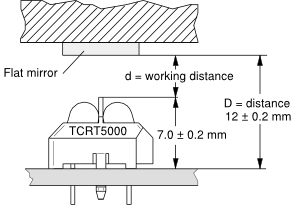
\includegraphics[width=0.5\textwidth]{reflex_test-circuit.png}%
    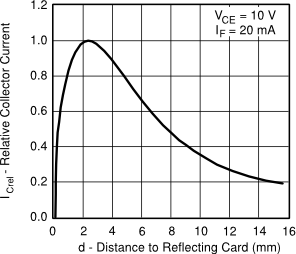
\includegraphics[width=0.5\textwidth]{reflex_working-distance.png}%
    \end{center}

    (α): \fullcite[3]{vishay09:test-circuit}

    (β): \fullcite[4]{vishay09:working-distance}
\end{figure}

Για τις ανάγκες της συσκευής, επιλέγεται λειτουργική απόσταση 2.5~cm έτσι ώστε ο
συντελεστής σύζευξης να ευνοείται όσο το δυνατόν περισσότερο.

\subsubsection{Διάστημα εναλλαγής}

Για τις ανάγκες της υλοποίησης, ο άξονας περιστροφής επικαλύπτεται, στο ύψος του
αισθήτηρα, από διαδοχικά τμήματα υψηλότερου και χαμηλότερου συντελεστή
ανάκλασης. Καθώς ο άξονας περιστρέφεται, η ένταση ρεύματος του συλλέκτη
μεταβάλλεται από τη μέγιστη μέχρι την ελάχιστη δυνατή και αντίστροφα.
Ωστόσο, σύμφωνα με το εγχειρίδιο της \textcite{vishay06}, εάν το πάχος των
τμημάτων είναι πολύ μικρό, ενδέχεται οι εναλλαγές να μην εκδηλώνονται αισθητά
στην ένταση ρεύματος του συλλέκτη.

Στο σχήμα \ref{fig:reflex:switching-distance} παρουσιάζεται η ένταση ρεύματος
του συλλέκτη για δύο διαδοχικά τμήματα.
Το σημείο εναλλαγής από τον ένα συντελεστή ανάκλασης στον επόμενο σημειώνεται
με το $Xo$ ενώ με $I_{c1}$ και $I_{c2}$, η μέγιστη ένταση ρεύματος του
συλλέκτη όταν η κοινή επιφάνεια $g$ των οπτικών πεδίων πομπού και δέκτη
καλύπτεται πλήρως από τμήμα του αντίστοιχου συντελεστή.
Προκύπτει ότι, ενώ η μετάβαση από τον ένα συντελεστή στον επόμενο συμβαίνει
ακαριαία, η ένταση ρεύματος του συλλέκτη $I_C$ έχει αρχίσει να μειώνεται σε
προγενέστερη μετατόπιση, όταν ένα πρώτο τμήμα των αρχικά διαθέσιμων ακτίνων
αποκόπηκε από το δέκτη, και συνεχίζει να μειώνεται σταδιακά έως ότου το τμήμα με
το νέο συντελεστή έχει καλύψει πλήρως την περιοχή $g$.

Επίσης, συμπαιρένεται ότι, καθώς το πάχος των τμημάτων μειώνεται ώστε η περιοχή
$g$ να είναι αδύνατο να καλυφθεί εξ ολοκλήρου από ένα μόνο τμήμα, η μέγιστη και
ελάχιστη τιμή έντασης ρεύματος που είναι δυνατό να σημειωθούν αρχίζουν να
συγκλίνουν, εφόσον, πλέον, σε κάθε μετατόπιση καταφθάνουν στο δέκτη ακτίνες από
όλο και περισσότερα τμήματα.

Το ελάχιστο πάχος τμημάτων καθορίζεται από το
\emph{διάστημα εναλλαγής}\index{διάστημα εναλλαγής} (\emph{switching distance}),
$X_d$, το οποίο ορίζεται ως το διάστημα μεταξύ δύο διαδοχικών τμημάτων
διαφορετικών συντελεστών ανάκλασης στο οποίο παρατηρείται το 90~\% $I_{C_1}$ έως
το 10~\% $I_{C2}$ \parencite{vishay06}. Η τιμή του διαστήματος εναλλαγής
εξαρτάται, από την κατασκευή του αισθητήρα καθώς και τη λειτουργική απόσταση,
ενώ όσο πιο μικρή απόσταση εναλλαγής υποστηρίζει κάποιος αισθητήρας, τόσο
υψηλότερη η διακριτική ικανότητά (resolution) του
\parencites{vishay02}{vishay06}. Για τον αισθητήρα TCRT5000, το διάστημα
εναλλαγής ανέρχεται στα 1.9~mm \parencite{vishay02}.

\begin{figure}
    \caption{Σχέση μεταβολής ρεύματος $I_C$ και συντελεστή ανάκλασης.
    \label{fig:reflex:switching-distance}}
    \begin{center}%
    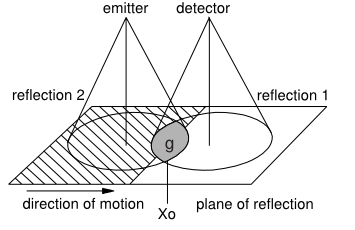
\includegraphics[width=0.4\textwidth]{reflex_switching-distance_a.png}%
    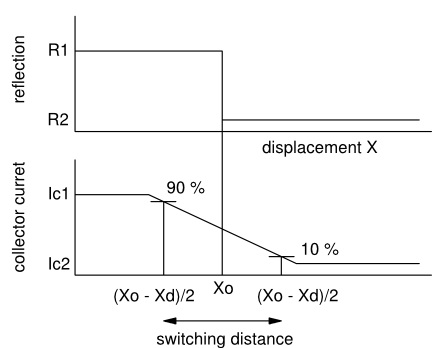
\includegraphics[width=0.5\textwidth]{reflex_switching-distance_b.png}%
    \end{center}

    \fullcite[3]{vishay06:switching-distance}
\end{figure}

\subsubsection{Συχνότητα αποκοπής}

Το φωτοτρανζίστορ---το πιο αργό στοιχείο του αισθητήρα---απαιτεί κάποιο χρόνο
για να ανταποκριθεί στις απότομες εναλλαγές έντασης των προσπίπτουσων ακτίνων
\parencite{vishay06}. Ως αποτέλεσμα, αν οι νέες εναλλαγές προκύπτουν πρωτού η
έξοδος του να έχει κατασταλάξει για μία προηγούμενη εναλλαγή, τότε η αναγνώρισή
τους καθιστάται μάλλον αβέβαιη. Άμεση απόρροια αυτού, δηλαδή του χρόνου
απόκρισης του φωτοτρανζίστορ, είναι η ανάγκη προσδιορισμού μίας μέγιστης
επιτρεπόμενης συχνότητας εναλλαγής των τμημάτων διαφορετικού συντελεστή
ανάκλασης ώστε να μην επηρεάζεται δραματικά ο συντελεστής σύζευξης. Η συχνότητα
αυτή αναφέρεται ως \emph{συχνότητα αποκοπής} \index{συχνότητα αποκοπής}
(\emph{cut-off frequency}) και είναι η συχνότητα στην οποία παρατηρείται μείωση
περίπου 30~\% του συντελεστή σύζευξης \parencite{vishay02}.

Το σχήμα \ref{fig:reflex:cutoff-frequency} παρουσιάζει πώς επηρεάζουν η τάση και
η αντίσταση φόρτου, $R_L$, του φωτοτρανζίστορ τη συχνότητα αποκοπής του
αισθητήρα.
Θα μπορούσε να χρησιμοποιηθεί χαμηλή τιμή αντίστασης φόρτου, ώστε να
μειωθεί ο χρόνος απόκρισης και, ως επέκταση, να διευρυνθεί το όριο της
συχνότητας αποκοπής. Ωστόσο, μία τέτοια κίνηση θα είχε ως αποτέλεσμα τη
μείωση της τάσης του παραγώμενου σήματος \parencite{vishay06}.
Προτιμάται να χρησιμοποιηθούν οι απαιτήσεις της υλοποίησης, όπως μέγιστη
ταχύτητα περιστροφής, για τον προσδιορισμό της συχνότητας αποκοπής και, μέσω
αυτής, της αντίστασης φόρτου.

\begin{figure}
    \caption{Σχέση Συχνότητας αποκοπής και Αντίστασης φόρτου.
    \label{fig:reflex:cutoff-frequency}}
    \begin{center}%
    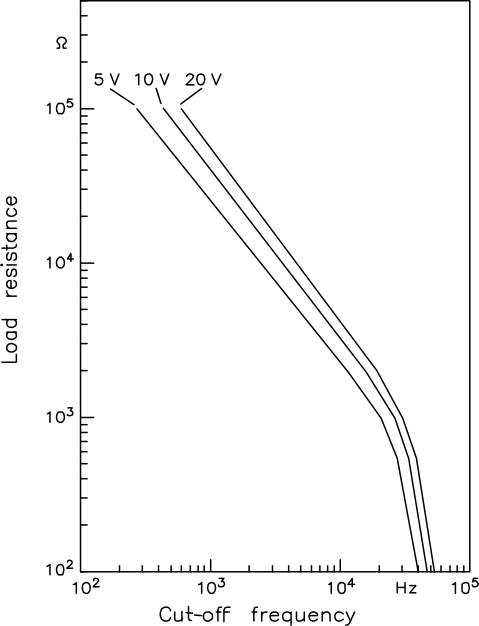
\includegraphics[width=0.5\textwidth]{reflex_cutoff-frequency.png}
    \end{center}

    \fullcite[5]{vishay02:cutoff-frequency}
\end{figure}

\subsubsection{Θερμοκρασία}
Η αύξηση θερμοκρασίας επηρεάζει την απόδοση τόσο της διόδου εκπομπής υπερύθρων,
η οποία μειώνεται, όσο και του φωτοτρανζίστορ, η οποία αυξάνεται
\parencite{vishay06}. Ωστόσο, όπως προκύπτει από το σχήμα
\ref{fig:reflex:t-amb_ctr-rel}, για θερμοκρασίες από -10~°C έως 70~°C, το
συνολικό αποτέλεσμα επηρεάζεται ελάχιστα. Θα μπορούσε, είτε να αγνοηθεί
πλήρως είτε να συμπεριληφθεί ως σταθερή μείωση του σχετικού λόγου μεταφοράς
ρεύματος.

\begin{figure}
    \caption{Σχέση θερμοκρασίας και Λόγου μεταφοράς ρεύματος.
    \label{fig:reflex:t-amb_ctr-rel}}
    \begin{center}%
    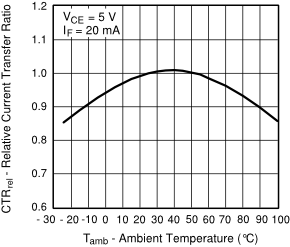
\includegraphics[width=0.5\textwidth]{reflex_t-amb_ctr-rel.png}
    \end{center}

    \fullcite[3]{vishay09:test-circuit}
\end{figure}

\subsection{Λοιπές παράμετροι}

\subsubsection{Ρεύμα ηρεμίας}

Ένα φωτοτρανζίστορ διαρρέεται από ρεύμα ακόμα και όταν αυτό βρίσκεται πλήρως
απομονωμένο από φωτεινές πηγές. Το ρεύμα αυτό αναφέρεται ως \emph{ρεύμα ηρεμίας}
\index{ρεύμα ηρεμίας} (\emph{dark current}) και επηρεάζεται από την τιμή της
τάσης συλλέκτη-εκπομπού, $V_{CE}$, και, σε μεγαλύτερο βαθμό, από τη θερμοκρασία
\parencite{vishay06}. Τυπική τιμή ρεύματος ηρεμίας, $I_{CEO}$, για τον αισθητήρα
TCRT5000 είναι τα 10~nA στα 20~V \parencite{vishay09}.

Κρίνεται σκόπιμο να αγνοηθεί στο σχεδιασμό εφόσον προκύψει από τους υπολογισμούς
ότι το ρεύμα ηρεμίας έντασης περίπου 5~μA που προκαλείται από την εφαρμογή
τάσης 10~V σε μία οριακή θερμοκρασία, $T_{amb}$, 100~°C, επηρεάζει ελάχιστα την
έξοδο του αισθητήρα (σχήμα \ref{fig:reflex:t-amb_i-ceo}).

\begin{figure}
    \caption{Σχέση θερμοκρασίας και Ρεύματος ηρεμίας.
    \label{fig:reflex:t-amb_i-ceo}}
    \begin{center}%
    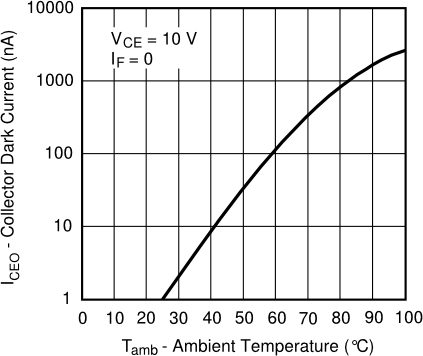
\includegraphics[width=0.5\textwidth]{reflex_t-amb_i-ceo.png}
    \end{center}

    \fullcite[3]{vishay06:dark-current}
\end{figure}

\subsubsection{Οπτικές παρεμβολές}

Σύμφωνα με τον οδηγό \textcite{vishay06}, είναι δυνατό να διοχετεύονται
εκπεμπόμενες ακτίνες από τον πομπό στο δέκτη απευθείας μέσα από την ίδια τη θήκη
καθώς και δια μέσω επιφανειών που περιβάλλουν τον αισθητήρα, πέραν της
ανακλαστικής επιφάνειας, με αποτέλεσμα να προκύπτει ένταση ρεύματος συλλέκτη.

Επιπλέον, σταθερή απευθείας πρόσπτωση φωτός στο φωτοτρανζίστορ μειώνει την
ευαισθησία του, δυνατό φως είναι δυνατό να το κρατήσει μονίμως ενεργό, ενώ
μεταβαλλόμενο, να προκαλέσει αδικαιολόγητη εναλλαγή στο σήμα εξόδου
\parencite{vishay06}.
Ο επιλεγμένος αισθητήρας διαθέτει προστατευτικά φίλτρα τα οποία παρεμποδίζουν το
ορατό φως \parencite{vishay09}. Ωστόσο, ένα μεγάλο εύρος του ηλιακού φωτός
αποτελείται από υπέρυθρες και, συνεπώς, η παράμετρος πρέπει να ληφθεί υπόψη κατά
το σχεδιασμό του συστήματος.

Η περίπτωση παρεμβολών που οφείλονται στην κατασκευή του αισθητήρα είναι δυνατό
να απαλειφθούν καταμετρώντας το σήμα του αισθητήρα σε πλήρη απομόνωσή του και
λαμβάνοντάς το υπόψη, ως σταθερά, κατά την κανονική λειτουργία του κωδικοποιητή.
Ο βαθμός στον οποίο επηρεάζουν οι περιβάλλουσες επιφάνειες μπορεί να εντοπιστεί
με παρόμοιο τρόπο. Ο βαθμός στον οποίο επηρεάζουν οι επικρατούσες συνθήκες
φωτισμού είναι, σαφώς, μεταβλητός και η ίδια προσέγγιση μη εφαρμοστέα. Ωστόσο,
είναι δυνατό να περιοριστεί απομονώνοντας εξωτερικά ολόκληρο τον κωδικοποιήτή,
δηλαδή αισθητήρα και ανακλαστική επιφάνεια.

\subsubsection{Θερμοκρασία}

Σε προηγούμενη παράγραφο, μελετήθηκε πώς επηρεάζει η θερμοκρασία το συντελεστή
σύζευξης. Ωστόσο, η θερμοκρασία θέτει και ορισμένα άλλα ζητήματα προς μελέτη.

Η αύξηση θερμοκρασίας της διόδου, ως άμεσο υποπροϊόν της κατανάλωσης ισχύος,
παίζει καθοριστικό ρόλο στον προσδιορισμό της έντασης ρεύματος της διόδου.
Σύμφωνα με το εγχειρίδιο χρήσης τους αισθητήρα \parencite{vishay09}, η μέγιστη
επιτρεπτή τιμή ρεύματος ορθής φοράς του πομπού, $I_F$, ανέρχεται στα 60~mA σε
θερμοκρασία περιβάλλοντος χώρου, $T_{amb}$, 25~°C. Επιπλέον, καθώς η θερμοκρασία
αυξάνεται, το μέγιστο επιτρεπτό όριο μειώνεται.
Το σχήμα \ref{fig:reflex:power-dissipation} δίνει την απόλυτη μέγιστη τιμή
κατανάλωσης ισχύος σε σχέση με τη θερμοκρασία. Λαμβάνοντας υπόψη ότι $P = VI$,
είναι δυνατό να υπολογιστεί το μέγιστο επιτρεπτό ρεύμα ορθής φοράς βάσει των
διακυμάνσεων της θερμοκρασίας χώρου και της εφαρμοζόμενης τάσης της υλοποίησης.

\begin{figure}
    \caption{Σχέση Κατανάλωσης ισχύος και Θερμοκρασίας.
    \label{fig:reflex:power-dissipation}}
    \begin{center}%
    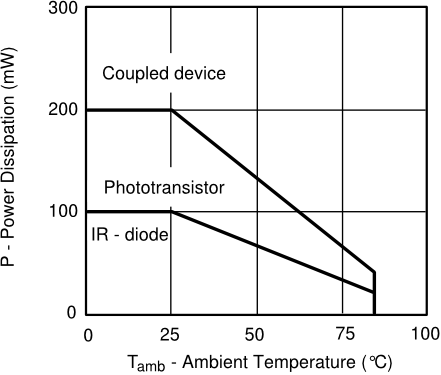
\includegraphics[width=0.5\textwidth]{reflex_power-dissipation.png}
    \end{center}

    \fullcite[3]{vishay09:power-dissipation}
\end{figure}

Κρίνεται αναγκαία η τήρηση χαμηλών θερμοκρασιών στη δίοδο για την επιμήκυνση της
ζωής της και, συνεπώς, του ίδιου του αισθητήρα, καθώς χαμηλή θερμοκρασία
συνεπάγεται ελάχιστη ή καθόλου φθορά της ένωσης p-n της διόδου. Προς επίτευξη
αυτού, η παρεχόμενη ένταση ρεύματος της διόδου είναι κατά πολύ μικρότερη από τη
μέγιστη αποδεκτή, κατάλληλη ακόμα και για θερμοκρασίες που ξεπερνούν τις
απαιτήσεις της υλοποίησης. Επίσης, ο αισθητήρας τίθεται σε λειτουργία μόνο για
τα διαστήματα περιστροφής του άξονα κίνησης, ώστε ο χρόνος κατανάλωσης ενέργειας
με αποτέλεσμα την εκπομπή θερμότητας και αύξηση της θερμοκρασίας τοπικά του
αισθητήρα να είναι περιορισμένος.

\chapter{Συνδεσμολογία}








\subsection{Πλατφόρμα Arduino}
\label{subsec:arduino}

Οι πλακέτες Arduino επιλύουν τα παραπάνω ζητήματα και παρέχουν μία έτοιμη
λειτουργική μονάδα που επιτρέπει την άμεση ενασχόληση με τη δημιουργία του
πρότυπου λογισμικού και εκείνων των συνδέσεων με ηλεκτρονικά στοιχεία που
απαιτούνται στο πλαίσιο αυτού.

Για την ύπαρξη αρκετής ευελιξίας κατά το σχεδιασμό της υλοποίησης (και λόγω
έλλειψης πρότερης εμπειρίας και, επομένως, κρίσης), επιλέγεται η (πλέον
πρόσφατη, την περίοδο εκπόνησης) πλακέτα Arduino Uno revision 3, της οποίας ο
κεντρικός μικροελεγκτής είναι ένας AVR ATmega328P της Atmel. Ο συγκεκριμένος
μικροελεγκτής διαθέτει συνολική μνήμη προγράμματος 32KiB, 2KiB κύρια μνήμη,
συχνότητα ρολογιού που φτάνει τα 20MHz (που, ωστόσο, λόγω της πλακέτας,
περιορίζεται στα 16MHz) και πληθώρα δυνατοτήτων
\parencites[1]{atmel13}{arduino:uno}. Επιπροσθέτως, η πλακέτα παρέχει διασύνδεση
USB για την επικοινωνία του μικροελεγκτή με τον υπολογιστή, τόσο για τον
προγραμματισμό του όσο και για την ανταλλαγή δεδομένων με κάποια άλλη εφαρμογή,
για παράδειγμα τερματικό.

Ο μικροελεγκτής της πλακέτας \te{Arduino Uno revision 3} διατίθεται με
προεγκατεστημένο
λογισμικό \te{Boot loader} επιτρέποντας, με αυτόν τον τρόπο, τον προγραμματισμό
της μνήμης προγράμματος χωρίς τη χρήση ειδικού υλικού, αλλά με την απευθείας
σύνδεση της πλακέτα μέσω καλωδίου USB \parencite{arduino:environ}. Περισσότερα
σχετικά με το λογισμικό \te{Boot loader} αναφέρονται στην ενότητα
\nameref{subsec:avr:progmem} σ.~\pageref{subsec:avr:progmem}.
Ωστόσο, σημειώνεται ότι η
επικοινωνία μέσω USB επιτυγχάνεται με ένα δεύτερο μικροελεγκτή της πλακέτας --
ενός ATmega16U2 -- του οποίου μοναδικός σκοπός είναι η διασύνδεση του
πρωτοκόλλου USB (το οποίο υποστηρίζει εγγενώς) με το κύκλωμα USART που διαθέτει,
τόσο ο ίδιος, αλλά, κυρίως, ο ATmega328P -- ο κεντρικός μικροελεγκτής της
πλακέτας \parencites{arduino:uno}[148,185]{atmel12}[172]{atmel13}. Σαφώς, αυτή η
διασύνδεση χρησιμοποιείται για κάθε επικοινωνία μεταξύ υπολογιστή και πλακέτας
μέσω καλωδίου USB, ανεξαρτήτως εάν τα δεδομένα προορίζονται για το λογισμικό
\te{Boot loader} ή το ίδιο το πρόγραμμα.

Για την περαιτέρω διευκόλυνση της ανάπτυξης του λογισμικού του μικροελεγκτή της
πλακέτας,
παρέχεται ορισμένο επιπρόσθετο λογισμικό \te{Arduino} το οποίο λαμβάνει δύο
μορφές. Μία εξ αυτών είναι το περιβάλλον ανάπτυξης \te{Arduino IDE} του οποίου
οι βασικές λειτουργίες είναι η μεταγλώττιση του πηγαίου κώδικα και η μεταφορά
του προγράμματος στο μικροελεγκτή \parencite{arduino:environ} μέσω μίας
περισσότερο ελκυστικής γραφικής διεπαφής. Μία δεύτερη μορφή
λογισμικού είναι οι βιβλιοθήκες \te{Arduino} οι οποίες παρέχουν εύχρηστες
προγραμματιστικές διεπαφές (API) που εσωτερικά κάνουν χρήση των υποκείμενων
κυκλωμάτων του μικροελεγκτή της εκάστοτε πλακέτας (είτε απευθείας, είτε μέσω
τρίτου λογισμικού) αποκρύπτοντας, με αυτόν τον τρόπο, τις λεπτομέρειες της
υλοποίησης \parencite{arduino:lib}.


\subsection{Περιβάλλον ανάπτυξης της υλοποίησης}

Παρότι το IDE και οι βιβλιοθήκες Arduino μπορούν να επιταχύνουν σημαντικά τη
διαδικασία ανάπτυξης της υλοποίησης, προτιμάται, αντί αυτών, η απευθείας χρήση
καθιερωμένων εργαλείων για τον προγραμματισμό μικροελεγκτών AVR, καθώς έτσι
επιδιώκεται να επιτευχθεί σε μεγαλύτερο βάθος κατανόηση της συνολικής
διαδικασίας που, ιδανικά, θα επιτρέψει τη μελλοντική ενασχόληση με παρόμοια
συστήματα ανεξαρτήτως της πορείας των προϊόντων \te{Arduino}. Στο πλαίσιο της
υλοποίησης, χρησιμοποιείται μόνο το υλικό, δηλαδή η πλακέτα \te{Arduino} για την
κάλυψη των βασικών ηλεκτρικών αναγκών, και το λογισμικό \te{Boot loader} για τον
προγραμματισμό του μικροελεγκτή.

Το IDE αντικαθίσταται από έναν οποιοδήποτε επεξεργαστή κειμένου και ο πηγαίος
κώδικας διασπάται σε διαφορετικά αρχεία για την καλύτερη οργάνωσή του.
Με τον τρόπο αυτό, καθώς η υλοποίηση επεκτείνεται και ο κώδικάς της διογκώνεται,
ο λογικός διαχωρισμός των λειτουργιών της επιτρέπει το γρηγορότερο εντοπισμό
κάποιας συγκεκριμένης υπομονάδας. Επιπλέον, καθώς η μεταγλώττιση μεγάλου όγκου
πηγαίου κώδικα μπορεί να αποβεί χρονοβόρα, η ύπαρξη αυτόνομων αρχείων
αντικείμενου κώδικα δημιουργημένων από προηγούμενο κύκλο μεταγλώττισης,
επιτρέπει την επαναχρησιμοποίησή τους για την παραγωγή ενός (νέου) συνολικού
δυαδικού αρχείου, απαιτώντας μεταγλώττιση μόνο των αρχείων εκείνων που έχουν
τροποποιηθεί.


\subsubsection{Εργαλεία AVR GCC}

Η μεταγλώττιση των επιμέρους αρχείων πηγαίου κώδικα σε αντικείμενα προγράμματα
και η, εν συνεχεία, σύνδεση (ή συνένωσή) τους σε ένα τελικό δυαδικό αρχείο
αναλαμβάνεται από την AVR GNU συλλογή μεταγλωττιστών avr-gcc και λοιπών
εργαλείων της avr-binutils (όπως ο συνδέτης ld ο οποίος χρησιμοποιείται
εσωτερικά από την avr-gcc).

Το παραγόμενο δυαδικό αρχείο της σύνδεσης είναι μορφής ELF (\te{Executable and
Linking Format}) η οποία, παρότι παρέχει ανεξαρτησία από επεξεργαστή και
αρχιτεκτονική υπολογιστή, είναι, ωστόσο ακατάλληλη για την απευθείας μεταφορά
στο μικροελεγκτή AVR \parencites[47]{cruz97}[346]{avrlibc}. Απαιτείται, πρώτα, η
εξαγωγή των τμημάτων (\te{segment}) του κώδικα και των δεδομένων (\@.\te{text}
και \@.\te{data}, αντίστοιχα) από το αρχείο ELF σε ένα αρχείο δεκαεξαδικής
μορφής (αρχείο HEX) · εργασία η οποία αναλαμβάνεται από το εργαλείο avr-objcopy
\parencite[13,346]{avrlibc}.

\begin{figure}
    \caption{Η αλυσίδα εργαλείων AVR GCC για τον προγραμματισμό του
    μικροελεγκτή.\label{fig:avr:toolchain}}
    \begin{center}
    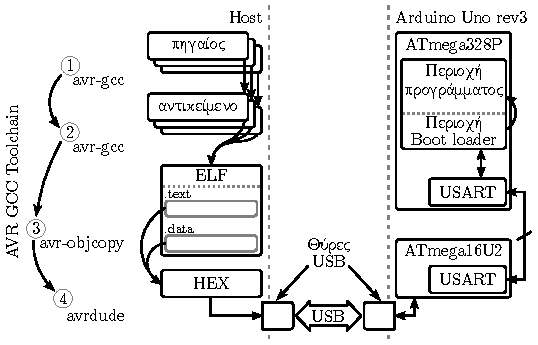
\includegraphics{avr_toolchain}
    \end{center}
\end{figure}

Τέλος, το δεκαεξαδικό αρχείο περνάει στο μικροελεγκτή μέσω του εργαλείου
avrdude, το
οποίο υποστηρίζει προγραμματισμό μικροελεγκτών AVR μέσω διαφόρων προγραμματιστών
(συμπεριλαμβανομένου ειδικών εξαρτημάτων όπως οι STK500 και AVRISP mkII της
Atmel) και, σαφώς, μέσω \te{Boot loader} \parencites[15]{avrlibc}{avrdude}.


\subsubsection{Εντολές προγραμματισμού}

Στο σχήμα \ref{fig:avr:toolchain} παρουσιάζεται η αλυσίδα (\te{toolchain}) των
χρησιμοποιούμενων εργαλείων για τη μετάβαση από κάθε στάδιο στο επόμενο με
τελικό στόχο τον προγραμματισμό του μικροελεγκτή. Στη βασική τους μορφή, οι
εντολές συνοψίζονται παρακάτω.

\begin{enumerate}

    \item Μετατροπή αρχείων πηγαίου σε αρχεία αντικείμενου κώδικα για κάθε
    αρχείο \verb~file.c~. Τυπικά, η εντολή εκτελείται μόνο για εκείνα τα αρχεία
    πηγαίου κώδικα που έχουν τροποποιηθεί.

\begin{lstlisting}
avr-gcc -mmcu=atmega328 -Wl,-Map,mcu.map -Os -c file.c
\end{lstlisting}

    \begin{description}
        \item[-mmcu] Καθορίζει τον τύπο του μικροελεγκτή ώστε να αναγνωρίζεται
        το κατάλληλο σύνολο εντολών (\te{instruction set}) που πρόκειται να
        χρησιμοποιηθεί κατά τη συμβολομετάφραση \parencite{gcc:options}.

        \item[-Os] Ενεργοποιεί τις βελτιστοποιήσεις του κώδικα από το
        μεταγλωττιστή προκειμένου να εξοικονομηθεί χώρος προγράμματος, ακόμα και
        εις βάρος της ταχύτητας εκτέλεσής του (Optimize for size)
        \parencites[338]{avrlibc}{gcc:options}.

        Εκτός του άμεσου πλεονεκτήματος της παραγωγής μικρότερου προγράμματος, η
        συγκεκριμένη ρύθμιση απαιτείται από τη βιβλιοθήκη AVR Libc προκειμένου
        να διατίθενται ορισμένες λειτουργίες προσωρινής «παύσης» της εκτέλεσης
        του προγράμματος (βρόχοι \te{busy-wait}) \parencite[328]{avrlibc}.

        \item[-c] Η συγκεκριμένη επιλογή προκαλεί την παραγωγή αρχείου
        αντικείμενου κώδικα όπως αυτό εξάγεται από το συμβολομεταφραστή,
        αποτρέποντας τη σύνδεσή του σε τελικό πρόγραμμα
        \parencites[338]{avrlibc}{gcc:options}.
    \end{description}


    \item Σύνδεση των αρχείων αντικείμενου κώδικα σε αρχείο ELF.
\begin{lstlisting}
avr-gcc -mmcu=atmega328 *.o -o mcu.elf
\end{lstlisting}

    \begin{description}
        \item[-mmcu] Ομοίως με την προηγούμενη εντολή.

        \item[-o] Καθορίζει το όνομα του παραγόμενου αρχείου
        \parencite{gcc:options}.
    \end{description}


    \item Μετατροπή αρχείου ELF σε δεκαεξαδική μορφή Intel HEX.
\begin{lstlisting}
avr-objcopy -j .text -j .data -O ihex mcu.elf mcu.hex
\end{lstlisting}

    \begin{description}
        \item[-j] Καθορίζει ποια τμήματα του αρχείου ELF θα χρησιμοποιηθούν για
        τη δημιουργία του αρχείου εξόδου. Στην προκειμένη, εξάγεται ο κώδικας
        και τα δεδομένα \parencite[346]{avrlibc}.

        \item[-O] Καθορίζει τον τύπο του παραγόμενου αρχείου
        \parencite[346]{avrlibc}. Στην περίπτωση του μικροελεγκτή AVR, πρόκειται
        για ένα αρχείο κειμένου ASCII του οποίου τα δεκαεξαδικά ψηφία
        κωδικοποιούν, ένα προς ένα, τα Byte του αρχικού δυαδικού αρχείου το
        οποίο αποτελεί το πρόγραμμα που εγγράφεται στη μνήμη Flash
        \parencites[4]{intel88}[10]{atmel12programmer}.
    \end{description}


    \item Αποστολή αρχείου HEX στο λογισμικό \te{Boot loader} του μικροελεγκτή
    για τη μετέπειτα εγγραφή του στην περιοχή προγράμματος (βλ.
    \nameref{subsec:avr:progmem} σ.~\pageref{subsec:avr:progmem}).
\begin{lstlisting}
avrdude -p atmega328p -c arduino -P /dev/ttyACM0 -b 115200 -U flash:w:mcu.hex:i
\end{lstlisting}
    \begin{description}
        \item[-p] Το μοντέλο του μικροελεγκτή, το οποίο στην περίπτωση της
        υλοποίησης είναι ο ATmega328P.

        \item[-c] Ο χρησιμοποιούμενος προγραμματιστής, ώστε να αναγνωρίζεται η
        συνδεσμολογία με το μικροελεγκτή και να εφαρμόζονται τα κατάλληλα
        σήματα ελέγχου.

        \item[-P] Η θύρα του υπολογιστή στην οποία είναι συνδεδεμένος ο
        προγραμματιστής. Στην περίπτωση της υλοποίησης όπου χρησιμοποιείται
        \te{Boot loader}, η θύρα σύνδεσης είναι USB η οποία, στο σύστημα του
        υπολογιστή, εμφανίζεται ως \slash{}dev\slash{}ttyACM0.

        \item[-b] Ο ρυθμός baud μετάδοσης δεδομένων μέσω της σειριακής. Σύμφωνα
        με τις προδιαγραφές του Arduino Uno, ο χρησιμοποιούμενος \te{Boot
        loader} λειτουργεί στα 115200Bd \parencite{arduino:environ}.

        \item[-U] Ο τύπος της εργασίας που πρόκειται να εκτελεστεί. Το πρόγραμμα
        avrdude μπορεί να χρησιμοποιηθεί τόσο για την εγγραφή όσο και για την
        ανάγνωση των διαθέσιμων μνημών του εκάστοτε μικροελεγκτή (για
        παράδειγμα, \te{Flash}, EEPROM, \te{fuse}), εφόσον αυτό υποστηρίζεται%
        \slash{}επιτρέπεται από τον μικροελεγκτή \parencite{avrdude}. Στο
        πλαίσιο της υλοποίησης, ενδιαφέρει μόνο η εγγραφή (\verb~w~) της μνήμης
        \te{Flash} με τα δεδομένα του αρχείου HEX (μορφής \verb~i~ntel).
    \end{description}

\end{enumerate}


\subsection{Λοιπό λογισμικό ανάπτυξης} % // Λοιπό υποστηρικτικό λογισμικό
% ή \subsubsection

Πέραν των εργαλείων της συλλογής AVR GCC που περιγράφονται στην ενότητα
\nameref{subsubsec:avr:toolchain} (σ.~\pageref{subsubsec:avr:toolchain}),
χρησιμοποιούνται και ορισμένα άλλα. Όλα πρόκειται για Ελεύθερο λογισμικό με τα
περισσότερα να υποστηρίζουν πολλαπλά λειτουργικά συστήματα πέραν των βασισμένων
σε \te{UNIX}.

% C spec as part of the GCC.

\begin{description}

% \nref{} : make
\item[Make]
Εργαλείο αυτοματισμού της ενημέρωσης παρακολουθούμενων αρχείων, αναγνωρίζει,
βάσει κανόνων που του δηλώνει ο χρήστης, ποια αρχεία έχουν τροποποιηθεί και
ενεργοποιεί τις αντίστοιχες εντολές για την ενημέρωσή αυτών καθώς και πιθανών
άλλων αρχείων εξαρτώμενων από αυτών που μόλις ενημερώθηκαν.

Στο πλαίσιο της
υλοποίησης, χρησιμοποιείται για την εκ νέου μεταγλώττιση μόνο εκείνων των
αρχείων πηγαίου κώδικα που έχουν τροποποιηθεί, παράγοντας τα αντίστοιχα αρχεία
αντικείμενου προγράμματος και την, εν συνεχεία, σύνδεσή τους για την παραγωγής
του αρχείου HEX. Επίσης, περιλαμβάνει τη μεταφορά του αρχείου στο μικροελεγκτή
καθώς και τη σύνταξη της τεκμηρίωσης (βλ. επόμενο εργαλείο).

%Εργαλείο που ορίζει συντακτικό βάσει του οποίου δηλώνει ο χρήστης 

\item[\LaTeX]
Σύστημα προετοιμασίας εγγράφων υψηλής τυπογραφικής αξίας, ορίζει ειδική σήμανση
κειμένου που χρησιμοποιείται για το χαρακτηρισμό του κειμένου και μέσω ορισμένων
εργαλείων, παράγεται το τελικό έγγραφο \parencite{latex}. Η παρουσίαση\slash{}%
εμφάνιση του εγγράφου (όπως περιθώρια, διατάξεις) καθορίζεται από,
τροποποιήσιμους έως ένα βαθμό, προκαθορισμένους εσωτερικούς κανόνες του
συστήματος \LaTeX{}  που έχουν δημιουργηθεί ώστε να ευνοείται η αναγνωσιμότητα
του τελικού προϊόντος.

Το σύστημα \LaTeX και τα σχετικά εργαλεία χρησιμοποιούνται για τη σύνταξη της
τεκμηρίωσης (του παρόντος εγγράφου). Μεταξύ άλλων, διευκολύνεται η εργασία με
αναφορές, τόσο μεταξύ μερών του εγγράφου όσο και των βιβλιογραφικών αναφορών και
η διατύπωση μαθηματικών παραστάσεων. Επίσης, καθώς ο επεξεργαστής κειμένου είναι
υπεύθυνος για την εμφάνιση μόνο κειμένου, η απόκριση του είναι ταχύτερη και ο
χειρισμός του πιο αποτελεσματικός.

Τέλος, επειδή τα αρχεία είναι κειμένου και όχι δυαδικά, οι αλλαγές που
πραγματοποιούνται σε αυτά είναι δυνατό να παρακολουθούνται από το σύστημα
παρακολούθησης αλλαγών σε επίπεδο γραμμής (βλ. επόμενο εργαλείο).

\item[Git]
Σύστημα παρακολούθησης αλλαγών το οποίο χαρακτηρίζεται για την ταχύτητα
τη μικρή επιβάρυνση σε πόρους συστήματος και την ευελιξία του \parencite{git}.
Επιτρέπει, μεταξύ άλλων, την καταγραφή των αλλαγών που πραγματοποιούνται σε
αρχεία της υλοποίησης (κατά κύριο λόγο, του πηγαίου κώδικα υλοποίησης και
τεκμηρίωσης) και παρέχει τη δυνατότητα πραγματοποίησης εύκολα αναστρέψιμων
πειραματικών αλλαγών.
Επιπλέον, παρέχει μία εύληπτη παρουσίαση πορείας των εργασιών που έχουν
πραγματοποιηθεί.

\item[Doxygen]
Λογισμικό παραγωγής τεκμηρίωσης πηγαίου κώδικα μέσω ειδικών σημάνσεων που
εισάγονται στα σχόλιά του, κυρίως απευθυνόμενο σε κώδικα γλώσσας C και C++
\parencite{doxygen}. Το σύνολο του πηγαίου κώδικα της υλοποίησης (για
παράδειγμα, συναρτήσεις, δομές, μεταβλητές) τεκμηριώνεται σύμφωνα με τις οδηγίες
του \te{Doxygen} ώστε να είναι δυνατή η δημιουργία ενός, ηλεκτρονικής μορφής,
προγραμματιστικού εγχειριδίου των επιμέρους μονάδων (\te{module}) για την
υποστήριξη της κατανόησης της λειτουργίας του καθενός και τη διευκόλυνση της
ενσωμάτωσης τους σε πιθανές άλλες υλοποιήσεις.

\item[Qucs]
Λογισμικό με γραφικό περιβάλλον (GUI) για τη δημιουργία και προσομοίωση
κυκλωμάτων, με δυνατότητα απεικόνισης των αποτελεσμάτων των προσομοιώσεων σε
διάφορες μορφές, όπως γραφήματα \parencite{qucs}.
Χρησιμοποιείται για το σχεδιασμό του προτύπου της διασύνδεσης του μικροελεγκτή
με όλα τα ολοκληρωμένα κυκλώματα και τα συμπληρωματικά στοιχεία της υλοποίησης.
Επιλέγεται, κυρίως, λόγω της ευκολίας με την οποία δημιουργούνται προσαρμοσμένα
κυκλώματα και επειδή υποστηρίζει την εξαγωγή των κυκλωμάτων σε διανυσματική
μορφή που εύκολα ενσωματώνεται στο έγγραφο της τεκμηρίωσης, δίχως απώλειες στην
ποιότητά τους.

\item[Inkscape]
Λογισμικό σχεδίασης διανυσματικών γραφικών \parencite{inkscape}. Χρησιμοποιείται
για τη δημιουργία όλων των επεξηγηματικών σχημάτων της τεκμηρίωσης για το λόγο
ότι επιτρέπει γρήγορη σχεδίαση γραφικών υψηλής ευκρίνειας με δυνατότητα εύκολης
ενσωμάτωσης στην τεκμηρίωση.

\item[Blender3D]
Ολοκληρωμένη σουίτα δημιουργίας τρισδιάστατων γραφικών \parencite{blender3d}.
Στο πλαίσιο της υλοποίησης, χρησιμοποιείται στο κομμάτι της κατασκευής της
συσκευής, τόσο για το σχεδιασμό και εξέταση προτύπων όσο και για την εξαγωγή
απεικονίσεων του εφαρμοσμένου προτύπου που περιλαμβάνονται, κυρίως, στο κεφάλαιο
\nameref{ch:construction} (σ.~\pageref{ch:construction}).

\item[Gimp]
Λογισμικό επεξεργασίας εικόνας \parencite{gimp}. Χρησιμοποιείται για τη βελτίωση
των χαρακτηριστικών ορισμένων εικόνων (για παράδειγμα, αντίθεση, κορεσμός), ώστε
να παρέχεται καλύτερο οπτικό αποτέλεσμα.
\end{description}


\section{Μικροελεγκτής}

Σύμφωνα με τον \textcite[1]{myklebust97}, οι μικροελεγκτές AVR διαθέτουν
μειωμένο σύνολο εντολών, δηλαδή είναι υπολογιστές RISC (\te{Reduced Instruction
Set Computer}). Το χαρακτηριστικό αυτό απλοποιεί τα απαιτούμενα κυκλώματα
ελέγχου και τους παρέχουν μικρότερους κύκλους για την εκτέλεση κάθε εντολής
\parencite[1]{sequin82}. Επιπροσθέτως, οι μικροελεγκτές AVR βασίζονται σε
τροποποιημένη αρχιτεκτονική Harvard σύμφωνα με την οποία, και σε αντίθεση με την
κατά Von Neumann αρχιτεκτονική, το πρόγραμμα και τα δεδομένα τοποθετούνται σε
ανεξάρτητα φυσικά μέσα που χαρακτηρίζονται, μεταξύ άλλων, από ανεξάρτητους
διαύλους πρόσβασης \parencite[1]{myklebust97}.

Άμεσα πλεονεκτήματα αυτού του σχεδιασμού είναι ότι καθίσταται δυνατή η
ταυτόχρονη πρόσβαση στις μνήμες προγράμματος και δεδομένων στον ίδιο κύκλο
\parencite[8]{atmel13}. Επιπλέον, επιτρέπεται η χρήση διαφορετικών τεχνολογιών
για κάθε μνήμη. Για παράδειγμα, στην περίπτωση του χρησιμοποιούμενου
μικροελεγκτή, ATmega328P, τα δεδομένα οργανώνονται σε μνήμη πλάτους των 8bit
τεχνολογίας SRAM (\te{Static RAM}) με 2KiB συνολική χωρητικότητα, ενώ οι
εντολές, σε μνήμη Flash των 32KiB με θέσεις των 16bit
\parencite[8--9,16,18]{atmel13}.


\subsection{Μνήμη προγράμματος}
\label{subsec:avr:progmem}

Η μνήμη Flash του μικροελεγκτή χωρίζεται σε δύο περιοχές λογισμικού, την περιοχή
του προγράμματος (\te{Application section}) και την περιοχή του λογισμικού
\te{Boot loader} (\te{Boot Loader Section} -- BLS) \parencite[269]{atmel13}.
Η περιοχή προγράμματος φέρει τον κώδικα που εκτελεί ο μικροελεγκτής κατά την
τυπική του λειτουργία· τον κώδικα της υλοποίησης. Στην περιοχή BLS εναποτίθεται
λογισμικό το οποίο μπορεί να εγγράψει και να διαβάσει τη μνήμη Flash με δεδομένα
που μεταφέρονται μέσω κάποιας διαθέσιμης διεπαφής του μικροελεγκτή (για
παράδειγμα, USART ή SPI), που, τυπικά, χρησιμοποιείται για την εναπόθεση του
νέου κώδικα του προγράμματος \parencite[269,273]{atmel13}.

Η εκτέλεση του \te{Boot loader} πραγματοποιείται είτε με την μεταπήδηση (εντολές
JMP ή CALL) στην περιοχή BLS από την περιοχή προγράμματος, είτε μέσω μίας
ρύθμισης του μικροελεγκτή που προκαλεί τη χρήση ως ρουτίνα εξυπηρέτησης της
διακοπής επανεκκίνησης (\te{Reset}), την πρώτη διεύθυνση της περιοχής BLS αντί
της πρώτης εντολής του προγράμματος, \parencite[273]{atmel13}. Από εκεί, το
λογισμικό \te{Boot loader} είναι υπεύθυνο να αποφασίσει εάν απαιτείται εγγραφή
νέου κώδικα στην περιοχή προγράμματος ή απευθείας μεταπήδηση πίσω σε αυτήν.

Το μέγεθος της περιοχής BLS είναι ρυθμιζόμενο και, στην περίπτωση του ATmega328,
δύναται να καταλαμβάνει τις τελευταίες 256, 512, 1024 ή 2048 λέξεις της μνήμης
Flash \parencite[282]{atmel13}. Στην περίπτωση του \te{Arduino Uno revision 3},
το λογισμικό \te{Boot loader} καταλαμβάνει 512KiB \parencite{arduino:uno}.


\subsection{Καθήκοντα μικροελεγκτή}

Κατά την εκκίνηση της συσκευής, δηλαδή κατά τη σύνδεσή της με την παροχή
τροφοδοσίας, εκτελείται η αρχικοποίηση των διαφόρων υποσυστημάτων της υλοποίησης
και, εν συνεχεία, ο μικροελεγκτής μεταπίπτει σε κατάσταση χαμηλής κατανάλωσης
ισχύος. Από αυτήν, ενεργοποιείται αυτόματα είτε για την εκκίνηση ενός νέου
κύκλου μετρήσεων (βλ. \nameref{sec:task} σ.~\pageref{sec:task}), είτε για την
εξυπηρέτηση κάποιου εισερχόμενου αιτήματος HTTP (βλ. \nameref{%
sec:network:impl-resources} σ.~\pageref{sec:network:impl-resources}). Στο σχήμα
\ref{fig:mcu:tasks} παρουσιάζεται ο κύκλος καθηκόντων του μικροελεγκτή.

\begin{figure}
    \caption{Καθήκοντα του μικροελεγκτή.\label{fig:mcu:tasks}}
    \begin{center}
    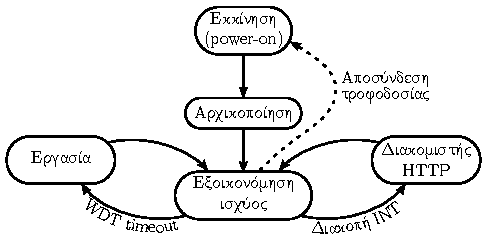
\includegraphics{mcu_tasks}
    \end{center}
\end{figure}

Αναλυτικότερα, κατά το στάδιο της αρχικοποίησης, τίθεται η συχνότητα του
ρολογιού του μικροελεκτή, η οποία, για τις ανάγκες της υλοποίησης, μειώνεται από
τα 16MHz στα 4MHz και η κατεύθυνση των ακροδεκτών (δηλαδή ποιοι είναι εισόδου
και ποιοι εξόδου). Επίσης, ρυθμίζεται το κύκλωμα WDT (\te{Watch-Dog Timer}), το
οποίο είναι υπεύθυνο για την περιοδική αφύπνιση του μικροελεγκτή ώστε να
ελέγχεται η ανάγκη εκκίνησης νέου κύκλου μετρήσεων.

Επιπλέον, ανακτώνται οι μεταβλητές ρυθμίσεις της συσκευής είτε από τις
προκαθορισμένες (εργοστασιακές ρυθμίσεις), είτε από τις αποθηκευμένες τιμές της
εφεδρικής μνήμης, εφόσον αυτές είναι έγκυρες (βλ \nameref{subsec:backup-memory}
σ.~\pageref{subsec:backup-memory}).
Οι ρυθμίσεις αυτές περιλαμβάνουν τη δικτύωση της συσκευής (διεύθυνση IP, μάσκα
υποδικτύου, προεπιλεγμένη πύλη), το λειτουργικό εύρος του υποσυστήματος κίνησης
(βλ. \nameref{sec:motor:coordinates} σ.~\pageref{sec:motor:coordinates}), το
χρονικό διάστημα μεταξύ κύκλων εργασίας καθώς και το πλήθος μετρήσεων που
πραγματοποιείται σε κάθε κύκλο (βλ. \nameref{sec:task} σ.~\pageref{sec:task}).
Ο τρόπος ρύθμισης της συσκευής περιγράφεται στους Πόρους υλοποίησης (σ.~%
\pageref{sec:network:impl-resources}).

Στην πορεία, οι ρυθμίσεις προωθούνται στις κατάλληλες μονάδες και εκτελούνται
επιπρόσθετες προετοιμασίες, όπως η παλιννόστηση της κεφαλής, δηλαδή η επαναφορά
της στη θέση επιστροφής (συντεταγμένες [0, 0, Z\tsub{max}]) (βλ. σ.~%
\pageref{sec:motor:homing}) και η αρχικοποίηση του HTTP \te{Socket} (βλ. σ.~%
\pageref{ssubsec:network:port_mr}).


\subsection{Κατάσταση χαμηλής κατανάλωσης}

Ο μικροελεγκτής διαθέτει διαφορετικές καταστάσεις νάρκης (\te{sleep mode}
όπου η καθεμία απενεργοποιεί ορισμένα κυκλώματα για τη μείωση της κατανάλωσης.
Για παράδειγμα, η πιο απλή, είναι η κατάσταση αδράνειας (\te{idle}) κατά την
οποία απενεργοποιείται μόνο το ρολόι της CPU και της μνήμης Flash (δηλαδή, της
μνήμης προγράμματος). Στο πλαίσιο της υλοποίησης, γίνεται προσπάθεια για την
ύψιστη μείωση της κατανάλωσης κατά τα διαστήματα όπου ο μικροελεγκτής παραμένει
άεργος.

Για το σκοπό αυτό, εφαρμόζεται η κατάσταση \te{power-down} κατά την οποία
απενεργοποιούνται όλα τα ρολόγια του μικροελεγκτή (clk\tsub{CPU}, clk%
\tsub{FLASH}, clk\tsub{IO}, clk\tsub{ADC}, clk\tsub{ASY}) καθώς και οι
ταλαντωτές του συστήματος και των Χρονομετρητών\slash{}Απαριθμητών \parencite%
[38]{atmel13}. Σύμφωνα με την \textcite[38]{atmel13}, ο μικροελεγκτής είναι
δυνατό να επανέλθει σε κανονική λειτουργία μόνο μέσω των ακροδεκτών INT1:0 με
παρατεταμένο λογικό 0 (\te{low-level interrupt}) καθώς και μέσω των κυκλωμάτων
TWI (\te{Two-Wire Interface}) και WDT (\te{Watch-Dog Timer}).

Στο πλαίσιο της υλοποίησης χρησιμοποιείται ο πρώτος και ο τελευταίος τρόπος· το
κύκλωμα TWI αφυπνίζει το μικροελεγκτή όταν αυτός ρυθμίζεται με ρόλο \te{slave}
στο δίαυλο TWI και κάποιο εξωτερικό κύκλωμα προσπαθεί να επικοινωνήσει μαζί του
ενώ, στην υλοποίηση, χρησιμοποιείται μόνο ως \te{master} για την επικοινωνία με
το ρολόι πραγματικού χρόνου (RTC) (βλ. \nameref{sec:rtc} σ.~\pageref{sec:rtc}).

Για την ακρίβεια, ο ένας εκ των δύο ακροδεκτών INT1:0 συνδέεται με τον ακροδέκτη
\nbar{INT} του ολοκληρωμένου δικτύωσης, W5100, το οποίο τον θέτει και τον
διατηρεί σε λογικό 0 έως ότου διευθετηθούν όλες οι ενδείξεις διακοπών που του
έχουν ενεργοποιηθεί
(βλ. \nameref{subsec:network:interface} σ.~\pageref{subsec:network:interface}).
Για τις ανάγκες της υλοποίησης, αυτό σημαίνει ότι έχει καταφθάσει εισερχόμενο
αίτημα HTTP το οποίο διεκπεραιώνεται από το διακομιστή (βλ.
\nameref{sec:http-server} σ.~\pageref{sec:http-server}).

Ο χρονομετρητής WDT ρυθμίζεται ώστε να αφυπνίζει το μικροελεγκτή κάθε 8s (το
μέγιστο διάστημα που υποστηρίζεται από τον παρόντα μικροελεγκτή) και αποτελεί το
έναυσμα για την εκκίνηση νέου κύκλου εργασιών
(\nameref{ssubsec:task:initiate} σ.~\pageref{ssubsec:task:initiate}).


\section{Η υλοποίηση συνοπτικά}


\subsection{Κατασκευή}

Η κατασκευή της συσκευής γίνεται με χρήση ανοικτού (\te{open hardware})
συστήματος κατασκευής (\te{construction framework}), το \te{Open\-Builds}, για
την παροχή διαφόρων διευκολύνσεων (ράγες κίνησης, γραμμική κίνηση).

Η συσκευή είναι εμπνευσμένη από τη διάταξη κινητού γεφυρώματος (\te{moving
gantry}) εργαλειομηχανών CNC για την επίλυση των αναγκών της για γραμμική κίνηση
στο χώρο, με εξαίρεση ότι αφαιρείται η τράπεζα.
%Οι διαστάσεις της συσκευής είναι
Η κίνηση αφορά την κεφαλή, ένα εξάρτημα που φέρει αισθητήρες, και μετακινείται
σε επίπεδο πάνω από την επιφάνεια του παρακολουθούμενο υλικού και κατακόρυφα
προς αυτό για την πραγματοποίηση μετρήσεων. Η ύπαρξη της κινητής κεφαλής
επιτρέπει την αξιοποίηση ενός μικρού αριθμού αισθητήρων για την κάλυψη όλου του
παρακολουθούμενου υλικού.


\subsection{Κωδικοποίηση κίνησης}

Η μετατόπιση της κεφαλής πραγματοποιείται από κινητήρες. Η κίνησή τους
παρακολουθείται από κωδικοποιητή περιστροφικής κίνησης, ο οποίος παρέχει
ανατροφοδότηση στο μικροελεγκτή για τα, αναφερόμενα ως, βήματα που πραγματοποιεί
ο παρακολουθούμενος κινητήρας ώστε να αναγνωρίζει το μέγεθος της μετατόπισης.
Τέσσερα τέτοια βήματα (ή παλμοί) αποτελούν μία πλήρη περιστροφή.

Ο κωδικοποιητής είναι αυτοσχέδιος και χρησιμοποιεί ανακλαστικό αισθητήρα
υπερύθρων ακτίνων· μέρος της έντασης των ακτίνων που εκπέμπει ο πομπός που
διαθέτει, καταφθάνουν στο δέκτη του, αφού πρώτα ανακλαστούν σε λωρίδες
εναλλασσόμενης ανακλαστικότητας που κοσμούν την άτρακτο του κινητήρα. Παρέχεται
ένας κωδικοποιητής ανά κινητήρα.

Η απόσταση του αισθητήρα από την άτρακτο καθώς και το πλάτος των λωρίδων
επιλέγονται σύμφωνα με τις προδιαγραφές του αισθητήρα ώστε να ευνοείται η
ικανότητά του να διακρίνει τις εναλλαγές.

Ο κωδικοποιητής λειτουργείται με χαμηλή ένταση ρεύματος και μόνο κατά τα
διαστήματα που κινείται ο αντίστοιχος κινητήρας για τη μείωση της συνολικής
κατανάλωσης ισχύος της συσκευής και για την επιμήκυνση της διάρκειας ζωής του
(πομπού του) αισθητήρα.


\subsection{Υποσύστημα κίνησης}

Η θέση της κεφαλής προσδιορίζεται από σύστημα συντεταγμένων τριών αξόνων X, Υ
και Z. Η ελάχιστη μετατόπιση ανά άξονα ορίζεται ως μία πλήρη περιστροφή της
ατράκτου του κινητήρα, πρακτικά 4cm.

Το σήμα ελέγχου της κίνησης των κινητήρων παράγεται μέσω κυκλώματος
Χρονομετρητή\slash{}Απαριθμητή (\te{Timer\slash{}Counter}) του μικροελεγκτή.
Η λήξη της κίνησης αναλαμβάνεται από δεύτερο κύκλωμα Χρονομετρητη\slash{}%
Απαριθμητή ο οποίος καταμετρά το πλήθος των βημάτων του κωδικοποιητή και
τερματίζει την αναμετάδοση του σήματος κίνησης στον κινητήρα όταν ολοκληρώνεται
το προκαθορισμένο πλήθος βημάτων. Η χρήση του δεύτερου κυκλώματος
Χρονομετρητή\slash{}Απαριθμητή επιτρέπει την παύση της μετατόπισης ακόμα και εάν
η CPU του μικροελεγκτή είναι απασχολημένη.

Υλοποιείται παράλληλη κίνηση της κεφαλής στους άξονες X και Y η οποία βασίζεται
στην παραδοχή ότι επιτυγχάνεται, και για τους δύο άξονες, η ίδια γωνιακή
ταχύτητα για το χρονικό διάστημα κατά τον οποίο λειτουργούν παράλληλα. Πρακτικά,
αυτό αποτελεί μία από τις προκλήσεις της υλοποίησης και χρήζει βελτίωσης, όπως
αναφέρεται και παρακάτω (\nameref{sec:improvements} σ.~%
\pageref{sec:improvements}).

Για την κάλυψη κάθε ενδεχομένου, χρησιμοποιούνται ανασταλτικοί διακόπτες στις
άκρες της συσκευής (όρια αξόνων). Όταν κάποιος εξ αυτών ενεργοποιηθεί, η κεφαλή
επαναφέρεται σε μία συγκεκριμένη θέση (την αρχική ή θέση επιστροφής). Από εκεί,
επιχειρείται μία ακόμη φορά η εκ νέου μετάβαση στην θέση που προηγουμένως
κατέστη αδύνατ. Εφόσον ενεργοποιηθεί κάποιος διακόπτης ξανά, η μετάβαση
ακυρώνεται.


\subsection{Μετρήσεις}

Η ύπαρξης της κεφαλής συνδέεται με την πραγματοποίηση μετρήσεων οι οποίες
αποθηκεύονται στην εσωτερική μνήμη EEPROM του μικροελεγκτή. Οι, κατά μέγιστο, 90
πλέον πρόσφατες καταγεγραμμένες μετρήσεις, φέρουν την ημερομηνία και τη θέση στο
επίπεδο X-Y όπου πραγματοποιήθηκε, καθώς και τη θερμοκρασία που σημειώθηκε.
Η ημερομηνία\slash{}ώρα παρέχεται από εξωτερικό ολοκληρωμένο ρολόι πραγματικού
χρόνου (RTC) το οποίο ρυθμίζεται από το χρήστη.

Η διαχείριση των εγγραφών γίνεται από τη μονάδα του ημερολογίου (\te{log}), η
οποία είναι υπεύθυνη και για τη διατήρηση της εγκυρότητας των περιεχόμενων
εγγραφών. Σε περίπτωση που πραγματοποιηθεί μέτρηση σε ημερομηνία προγενέστερη
(σύμφωνα με την ώρα του RTC) σε σχέση με υπάρχουσες εγγραφές, το ημερολόγιο
εγγράφει τη νέα μέτρηση αποβάλλοντας τις προϋπάρχουσες προγενέστερες (λογική
διαγραφή και όχι φυσική για την μείωση φθορών στην EEPROM).

Μετρήσεις πραγματοποιούνται αυτόματα από τη συσκευή ανά σταθερά χρονικά
διαστήματα καθοριζόμενων από το χρήστη, σε ένα πλήθος τυχαία επιλεγμένων θέσεων.
Το πλήθος των μετρήσεων καθορίζεται, επίσης, από το χρήστη. Μία σειρά μετρήσεων
αναφέρεται ως εργασία και ξεκινά σε διαστήματα πολλαπλάσια των έξι λεπτών της
ώρας. Ο μέγιστος χρόνος αδράνειας της συσκευής που υποστηρίζεται είναι, πέραν
της εξ ολοκλήρου απενεργοποίησης των εργασιών, μία ημέρα.


\subsection{Επικοινωνία με συσκευή}

Η επικοινωνία της συσκευής με εξωτερικές οντότητες γίνεται μέσω πρωτοκόλλου
HTTP· ο χρήστης αλληλεπιδρά μαζί της μέσω λογισμικού πλοήγησης (\te{browser})
ενώ τρίτα συστήματα, μέσω προγραμματιστικής διεπαφής (API).
Για την ακρίβεια, η ίδια η διεπαφή χρήστη αποτελεί έναν καταναλωτή αυτής της
προγραμματιστικής διεπαφής (API), και είναι υλοποιημένη με HTML5, CSS3 και
Javascript (χωρίς επιπρόσθετες βιβλιοθήκες) σε βαθμό ώστε να παρέχεται
συμβατότητα με τις περισσότερες εκδόσεις των δημοφιλέστερων λογισμικών πλοήγησης
και για εκδόσεις \te{Internet Explorer} 8 και άνω.

Τα δεδομένα που είναι απαραίτητα για τη διεπαφή του χρήστη (ιστοσελίδα και
αρχεία \@.css \@.js και εικόνων) εναποτίθενται σε εξωτερικό κύκλωμα μνήμης Flash
128KiB το οποίο χρησιμοποιείται μόνο για την ανάγνωσή τους και την επιστροφή
τους μέσω του υποσυστήματος διακομιστή HTTP.
Τα δεδομένα που ανταλλάσσονται μεταξύ τρίτων συστημάτων και συσκευής βρίσκονται
σε αναπαράσταση JSON (πέραν των HTML, CSS, Javascript και PNG που προορίζονται
για τη διεπαφή χρήστη).

Μέσω της διεπαφής της συσκευής δύναται η εμφάνιση των μετρήσεων που έχουν
πραγματοποιηθεί καθώς και οι ρυθμίσεις της συμπεριφοράς της. Οι ρυθμίσεις
διατηρούνται ακόμη και με την αποσύνδεση της συσκευής από την κεντρική
τροφοδοσία. Η επαναφορά τους στις εργοστασιακές (προκαθορισμένες) τιμές γίνεται
μέσω της προσωρινής απομάκρυνσης της μπαταρίας (\te{coin cell}) της συσκευής ενώ
αυτή είναι αποσυνδεδεμένη από την κεντρική τροφοδοσία.
Σημειώνεται ότι οι εργοστασιακές ρυθμίσεις απενεργοποιούν τις εργασίες, ενώ οι
ρυθμίσεις δικτύου είναι αυτές που ορίζονται στον πίνακα \ref{tab:default-ip}.

\begin{table}
    \caption{Εργοστασιακές ρυθμίσεις δικτύωσης της συσκευής.
    \label{tab:default-ip}}
    \begin{center}
    \begin{tabu} to 6cm {X[L] *3{X[-2.5,R] @{.}} X[-1,R]}

    {\bfseries Διεύθυνση IP} :
        & 192 & 168 &   1 & 73 \\
    {\bfseries Προεπιλεγμένη πύλη} :
        & 192 & 168 &   1 &  1 \\
    {\bfseries Μάσκα υποδικτύου} :
        & 255 & 255 & 255 &  0 \\
    \end{tabu}\end{center}
\end{table}

%Αντιστοίχιση όρων
%PWM	διαμόρφωση διάρκειας παλμών	Βιβλίο τηλεπικοινωνιών



\printbibliography[nottype=image,nottype=table]
\printindex
\end{document}
